\documentclass[border=12pt]{standalone}
\def\pgfsysdriver{pgfsys-dvisvgm.def}
\usepackage[dvisvgm]{xcolor}
\usepackage{xeCJK}
\setCJKmainfont{HaranoAjiGothic-Regular.otf}[BoldFont=HaranoAjiGothic-Bold.otf]
\setCJKsansfont{HaranoAjiGothic-Regular.otf}[BoldFont=HaranoAjiGothic-Bold.otf]
\usepackage{amsmath,amssymb,tikz,lmodern}
\usetikzlibrary{arrows.meta,positioning,calc,fit,backgrounds}
\renewcommand{\familydefault}{\sfdefault}
\definecolor{ink}{HTML}{25322F}
\definecolor{green}{HTML}{246657}
\definecolor{tint}{HTML}{EEF4F0}
\definecolor{soft}{HTML}{C6D2CC}
\definecolor{muted}{HTML}{52615B}
\newif\ifJapanese
\newcommand{\Tx}[2]{\ifJapanese #1\else #2\fi}
\newcommand{\Eff}{\overline{\operatorname{Eff}}}
\newcommand{\heading}[3]{{\color{green}\bfseries #1\quad\Tx{#2}{#3}}\\[5pt]}
% A white rectangle makes the complete citation label clickable, including spaces.
\newcommand{\refurl}[2]{\special{dvisvgm:raw <a xlink:href="#1" target="_blank" rel="noopener noreferrer">}{\setlength{\fboxsep}{0pt}\colorbox{white}{\color{green}\underline{\strut #2}}}\special{dvisvgm:raw </a>}}
\newcommand{\refedge}[3]{\refurl{\csname source#1\endcsname\string##page=#2}{#3}}
\newcommand{\SF}[2]{\refedge{sf}{#1}{#2}}
% GitHub's file preview does not support PDF page fragments.
\newcommand{\LA}[2]{\refurl{\sourcela}{#2}}
\newcommand{\Sch}[2]{\refedge{sch}{#1}{#2}}
\newcommand{\PS}[2]{\refedge{ps}{#1}{#2}}
\tikzset{
 card/.style={draw=soft,fill=white,rounded corners=2pt,align=left,text=ink,font=\fontsize{10.5}{14}\selectfont,inner xsep=12pt,inner ysep=10pt,text width=14.4cm},
 half/.style={card,text width=6.45cm,minimum height=2.05cm},
 result/.style={card,draw=green,fill=tint,line width=.9pt},
 reason/.style={align=left,text=muted,font=\fontsize{9}{12}\selectfont,inner sep=0pt,text width=12.7cm},
 branchreason/.style={reason,text width=5.95cm},
 edge/.style={-{Stealth[length=2.4mm]},draw=green,line width=1pt},
 wire/.style={draw=green,line width=1pt},
}
% Keep the arrow in a dedicated left gutter; explanations never cover it.
\newcommand{\flow}[3]{
 \coordinate (#2-from) at ($(#1.south)+(-6.9,0)$);
 \coordinate (#2-to) at ($(#2.north)+(-6.9,0)$);
 \draw[edge] (#2-from)--(#2-to);
 \node[reason,anchor=west] (#2-reason) at ($(#2-from)!.5!(#2-to)+(.55,0)$) {#3};
}


\newcommand{\CiteSource}[2]{\refurl{\csname source#1\endcsname}{#2}}

\expandafter\def\csname sourceRD\endcsname{https://github.com/openai/math/blob/adc7f1241b42e322a6451854ab7e4b4c146bf78a/preprints/Relative-denominators-and-effective-systems-for-log-Calabi-Yau-fibrations-September-27-2026/paper.pdf}
\expandafter\def\csname sourceSL\endcsname{https://github.com/openai/math/blob/adc7f1241b42e322a6451854ab7e4b4c146bf78a/preprints/Lifting-sections-from-the-reduced-support-of-an-adjoint-September-27-2026/paper.pdf}
\expandafter\def\csname sourceLA\endcsname{https://github.com/openai/math/blob/adc7f1241b42e322a6451854ab7e4b4c146bf78a/preprints/Log-abundance-in-characteristic-zero-September-24-2026/paper.pdf}
\expandafter\def\csname sourceJL\endcsname{https://arxiv.org/pdf/2002.11928v1}
\expandafter\def\csname sourceXu\endcsname{https://arxiv.org/pdf/1905.00297v2}
\expandafter\def\csname sourceCT\endcsname{https://arxiv.org/pdf/2011.02236v2}
\expandafter\def\csname sourceUfour\endcsname{https://github.com/openai/math/blob/adc7f1241b42e322a6451854ab7e4b4c146bf78a/preprints/Uniform-effective-log-Iitaka-fibrations-for-fourfolds-September-26-2026/paper.pdf}

\Japanesetrue
\begin{document}
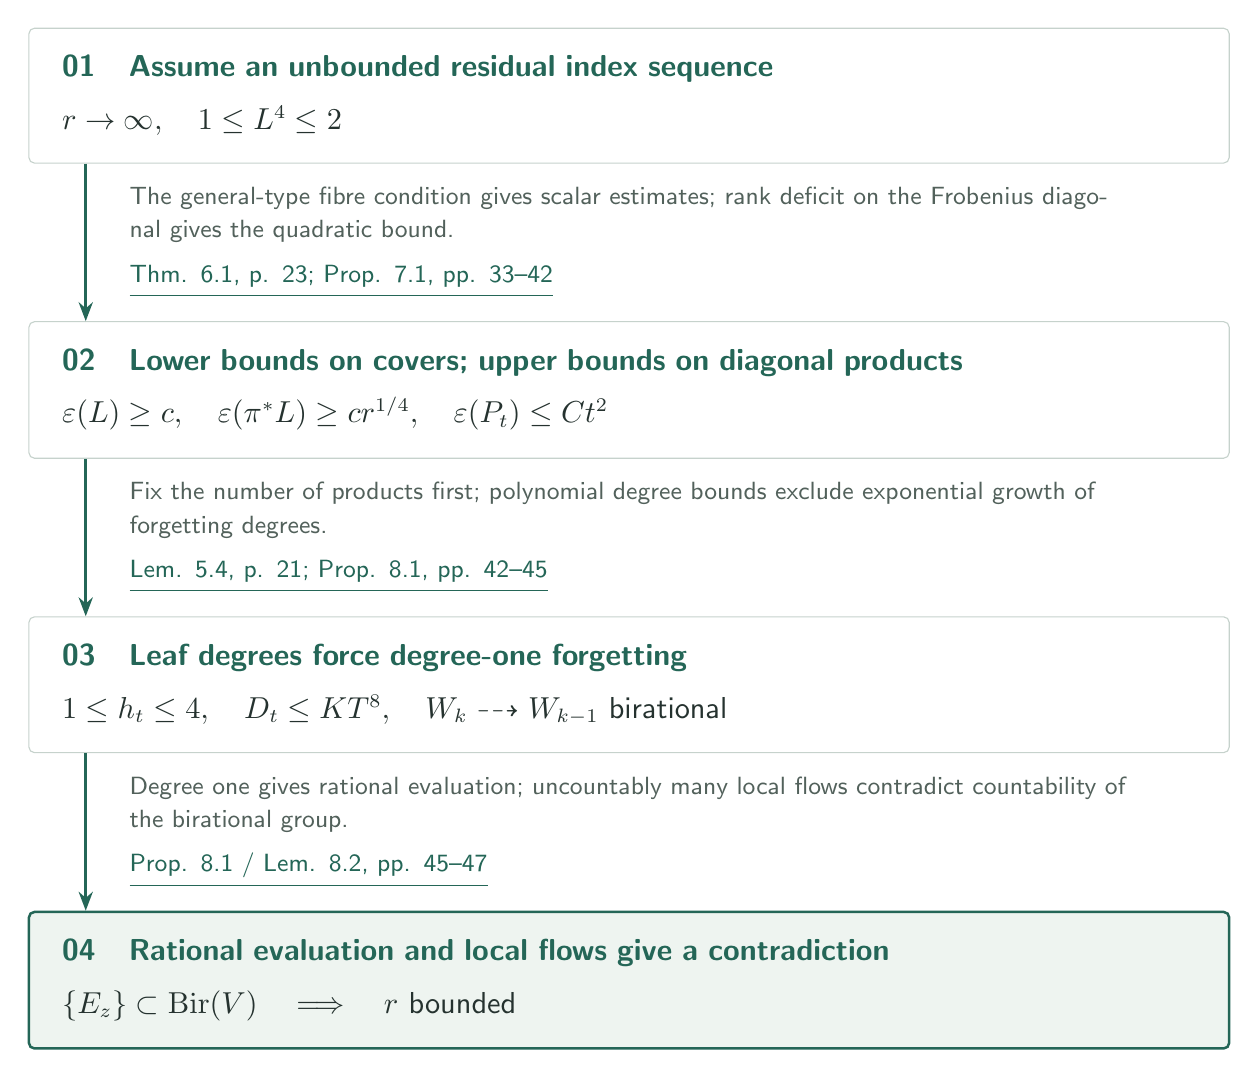
\begin{tikzpicture}
\node[card] (n0) {\heading{01}{指数が増大する残余列を仮定}{Assume an unbounded residual index sequence}$r\to\infty,\quad 1\leq L^4\leq2$};
\node[card,below=2.0cm of n0] (n1) {\heading{02}{被覆上の下界と対角積上の上界}{Lower bounds on covers; upper bounds on diagonal products}$\varepsilon(L)\geq c,\quad\varepsilon(\pi^*L)\geq cr^{1/4},\quad\varepsilon(P_t)\leq Ct^2$};
\flow{n0}{n1}{\Tx{一般型ファイバー条件からscalar評価。Frobenius対角の階数欠損で二次上界を得る。}{The general-type fibre condition gives scalar estimates; rank deficit on the Frobenius diagonal gives the quadratic bound.}\\[4pt]\CiteSource{Ufour}{Thm. 6.1, p. 23; Prop. 7.1, pp. 33--42}}
\node[card,below=2.0cm of n1] (n2) {\heading{03}{葉の次数と次数1の忘却}{Leaf degrees force degree-one forgetting}$1\leq h_t\leq4,\quad D_t\leq KT^8,\quad W_k\dashrightarrow W_{k-1}\text{ birational}$};
\flow{n1}{n2}{\Tx{先に積の個数を固定。鎖の次数を多項式で抑え、忘却次数の指数増大を排除する。}{Fix the number of products first; polynomial degree bounds exclude exponential growth of forgetting degrees.}\\[4pt]\CiteSource{Ufour}{Lem. 5.4, p. 21; Prop. 8.1, pp. 42--45}}
\node[result,below=2.0cm of n2] (n3) {\heading{04}{有理評価と局所流による矛盾}{Rational evaluation and local flows give a contradiction}$\{E_z\}\subset\operatorname{Bir}(V)\quad\Longrightarrow\quad r\text{ bounded}$};
\flow{n2}{n3}{\Tx{次数1が有理評価を与える。非可算個の局所流と双自己写像群の可算性が衝突する。}{Degree one gives rational evaluation; uncountably many local flows contradict countability of the birational group.}\\[4pt]\CiteSource{Ufour}{Prop. 8.1 / Lem. 8.2, pp. 45--47}}
\end{tikzpicture}
\end{document}
